% !TeX spellcheck = en_US
%===============================================================================
% $Id: ifacconf.tex 19 2011-10-27 09:32:13Z jpuente $
% Template for IFAC meeting papers
% Copyright (c) 2007-2008 International Federation of Automatic Control
%===============================================================================
\documentclass{ifacconf}

\usepackage{graphicx}      % include this line if your document contains figures
\usepackage{natbib}        % required for bibliography

\usepackage[utf8]{inputenc}

\usepackage{amsmath}
\usepackage{amssymb}
\usepackage{color}
\usepackage{datetime}
\usepackage{placeins}
\usepackage{textcomp}

%===============================================================================

\graphicspath{
{images/}
}

% Custom commands
\providecommand{\mbf}[1]{\mathbf{#1}}
\newcommand{\idxFollower}{{\ensuremath{i} }}
\newcommand{\idxPredecessor}{{\ensuremath{i-1} }}
\newcommand{\idxSample}{{\ensuremath{k}}}
\newcommand{\idxAxis}{{\ensuremath{p}}}
\newcommand{\Francois}{\mbox{Fran\c{c}ois Defa$\ddot{\textrm{y}}$}}

\begin{document}
\begin{frontmatter}

\title{Discrete Sliding Mode control of small UAS in tight formation flight under information constraints}
% Title, preferably not more than 10 words.

\author[First]{Jan Bolting}
\author[First]{Soheib Fergani}
\author[Second]{Jean-Marc Biannic}
\author[First]{Francois Defay}
\author[Second]{Martin Stolle}

\address[First]{Institut Supérieur de l'Aéronautique et de l'Espace (ISAE),
   31055 Toulouse, France (e-mail: jan.bolting@isae.fr, soheib.fergani@isae.fr, francois.defay@isae.fr)}
\address[Second]{Office National d'Études et de Recherches Aérospatiales (ONERA),
   31055 Toulouse, France (e-mail: jean-marc.biannic@onera.fr, martin.stolle@onera.fr)}
   
%\textcolor{red}{\Huge !!! DRAFT !!!\\ \normalsize \today \\ \currenttime}

% Abstract of not more than 250 words.
\begin{abstract}
This paper is concerned with a new control strategy  based on discrete sliding mode control of small Unmanned Aerial Systems (UAS) in tight formation flight under information constraints. 
Tight formation flight enables, among other advantages, significant performance benefits due to wake vortex interactions. 
%To benefit from other aircraft's wake vortices, follower aircraft need to remain inside a small spatial window behind their predecessor. Therefore high-performance relative position control becomes an important issue.
A discrete robust control strategy based on the sliding mode approach and a leader-follower scheme is proposed to achieve the desired flight performances while assuming realistic information constraints imposed by limited inter-vehicle communication bandwidth and availability of relative localization sensors.
% and preserving scalability with respect to formation size.
For the discrete sliding mode controller (DSMC), a novel predictive reaching law is proposed and compared to a linear reaching law. This predictive sliding mode control (PDSMC) strategy allows to avoid actuator saturation by solving an optimization problem at each time step.\\
Also, this paper presents a meaningful study and comparison of the two discrete sliding mode control designs and  time sampling continuous sliding mode control (TSCSMC). 
% Indeed, it is important to study the performance differences between the two approaches that allow to choose the best strategy to be used to solve the considered problem. 
Here, the comparison focuses on the effect of discrete sampling on the control error analytically and in simulation. Effects on mesh stability are evaluated in simulation.
Simulation results of a flight scenario with two different sampling frequencies demonstrate the efficiency of the proposed control strategy and show clearly the effect of the sampling time on the formation flight performance of the UAS obtained by the considered control strategies.

%It addresses the problem of managing and coordinating several UAS to fly in a tight formation. Since the formation of $n$ UAS to be controlled is considered to fly in an arbitrary pattern in this work, 


%Indeed, the capability of autonomous formation flight has the potential to significantly enhance the utility and efficiency of small low-cost UAS. Formations of small, inexpensive fixed-wing UAS allow for the sharing of remote sensing functionality, mission-level redundancy and range enhancements due to aerodynamic interactions widely exploited by migratory birds.
%
%The capability of autonomous formation flight has the potential to significantly enhance the utility and efficiency of small low-cost Unmanned Aerial Systems (UAS). Formations of small, inexpensive fixed-wing UAS allow for the sharing of remote sensing functionality, mission-level redundancy and range enhancements due to aerodynamic interactions widely exploited by migratory birds.
%For the latter application, high-performance relative position control is essential.
%This becomes challenging when assuming realistic information constraints imposed by limited communication bandwidth and availability of relative localization sensors,  while preserving scalability with respect to formation size.
%This article presents a Discrete Time Sliding Mode controller for tight formation flight and studies its
%
%State-based STCSMC\\
%State-based DSMC\\
%For both:\\
%Effects of sampling on control error\\
%Effects of sampling on mesh stability in simulation\\
%Effects of sampling on mesh stability analytically
\end{abstract}

\begin{keyword}
UAS, Formation flight, discrete sliding mode control, robust control.
\end{keyword}

\end{frontmatter}
%===============================================================================

\section{Introduction}
The capability of autonomous formation flight has the potential to significantly enhance the utility and efficiency of small low-cost UAS. 
Formations of small, inexpensive fixed-wing UAS allow for the sharing of remote sensing functionality, mission-level redundancy and range enhancements due to aerodynamic 
interactions widely exploited by migratory birds. 
%Aircraft formation flight can enhance the fuel efficiency thanks to the aerodynamics and the induced airflow by leading aircraft, in the same way that the migratory birds use some formation patterns. 
Indeed, in \cite{weimerskirch2001energy} authors have measured heart rates as an estimate of energy expenditure in imprinted great white pelicans (Pelecanus onocrotalus) trained to fly in 'V' formation, and show that these birds save a significant amount of energy by flying in formation. This advantage is probably a principal reason for the evolution of formation flight in large birds that migrate in groups.\\
\begin{figure}
\begin{center}
\includegraphics[width=\columnwidth,height=6cm]{juppmehrbionik}    % The printed column width is 8.4 cm.
\vspace{-1cm}
\caption{Formation flight: migrant birds inspiring aircraft performance evolution}
\label{fig:birds}
\end{center}
\end{figure}
%Also, this strategy has a lot of advantages as sharing of remote sensing functionality, mission-level redundancy, range enhancements due to aerodynamic interactions and energy saving. 
Based on that, the NASA AFF program has demonstrated the feasibility of this approach for manned fighter aircraft in a 2-aircraft configuration. Maximum fuel flow savings of $18\%$ for the follower are reported (\cite{Vachon2002}). This emphasizes the importance of formation flight since no structural changes have to be made to the aircraft to gain considerable fuel savings.\\
Recently, both academical and industrial communities have been very interested in the formation flight of manned aircraft and UAS. In \cite{wolfe1996decentralized}, decentralized control is presented to increase the efficiency of formation flight of five aircraft in a single line. These controllers are derived from a linear model and tested on a linear simulation incorporating a vortex-lattice aerodynamics routine. Another interesting study in \cite{thien2008effects} focuses on the effect of the leader's position and shape on aerodynamics performances of a given V flight formation. Vortices generated by the wing tip of the leader move downstream forming a pair of counter-rotating line vortices. Some interesting control solutions for autonomous formation flight were introduced in \cite{giulietti2000autonomous}. Moreover, in the last decade, a lot of researchers have focused on improving the control strategies to enhance the formation flight performance. A suitable control strategy for  controlling a team of micro-aerial vehicles moving quickly through a three-dimensional environment while maintaining a tight formation is presented in \cite{turpin2012trajectory}. Moreover, an interesting control performance analysis for autonomous close formation flight experiments has been achieved in \cite{rice2014control}.\\
In this paper, a discrete robust sliding mode control strategy is proposed to manage the formation flight of UAS. Indeed, sliding mode control has been proved as a very efficient implementable solution for ground vehicle platooning (see \cite{ferrara2008sliding} and \cite{zou2013distributed}). Also, the sliding mode control is a very efficient and robust approach regarding environmental disturbances to ensure good position tracking performances. 
Here, the authors provide a robust discrete sliding mode control solution to manage the tight formation flight of multiple UAS considering external disturbances due to atmospheric turbulence and the predecessor's wake. Then, a comparison between two discrete time sliding mode control strategies (Discrete sliding mode control (DSMC) with linear reaching law and Predictive Discrete Sliding Mode Control (PDSMC)) and the discretization of a time continuous sliding mode controller (Time Sampled Continuous Sliding Mode Control TSCSMC) from the literature is presented. Indeed, it proves that the discretization of the time continuous designed controller decreases the tracking performances and the robustness regarding environmental disturbances.
Both the DSMC and the PDSMC are shown to offer better tracking performances for realistic sampling times.\\
This paper is structured as follows: section \ref{sec:model} presents the aircraft model, section \ref{sec:controldesign} presents the TSCSMC, the DSMC, and the PDSMC controller designs, simulation results are given in section \ref{sec:simulations} and section \ref{sec:conclusion} provides a short summary and an outlook of future extensions to our approach.
\section{Model}
\label{sec:model}
\subsection{Coordinate frames}
The main objective of this work is to provide an efficient control strategy for a formation of $n$ UAS flying in an arbitrary pattern. It is assumed that load factors are tracked (by low level controllers) in each vehicle's body frame (index $b$). 
%Therefore separation errors are transformed into the body frame for control purposes, decoupling the three axes. 
The dynamics of each vehicle are defined in a local inertial North-East-Down frame (NED, index $e$). 
%It is convenient to note the relative separations of the vehicles in a frame that approximates the leader's wind frame (which is not available due to the absence of sensors for angle of attack and sideslip angle on small UAS). We define for this purpose the Follower Velocity frame (index $fv$). Its x axis is aligned with the follower's inertial speed projected on the horizontal plane, and its z axis is aligned with the NED frame's z axis. Its origin coincides with that of the predecessor's body frame. 

%The follower's wind frame would be preferable, since the lift vector is by definition aligned with its z axis , but requires on-line wind estimation or flow sensors that usually are not available on board small UAS. It is preferable over the Predecessor Velocity Frame (PF), since to form the rotation matrix between the FF and the inertial frame the predecessor's absolute velocity does not need to be communicated to the follower.

%The right choice of reference frames can significantly facilitate control design. To give one example, when performing navigation in the predecessor's body frame, variations in the predecessor's attitude will couple into follower's position control loops, increasing control action. What is more, the effect increases with inter-vehicle separation, leading to high control demands during the initial rendezvous maneuver. To avoid such disadvantages, the motion of the reference frame with respect to the inertial frame should be within the control bandwidth of the position controller. A suitable frame is a local Cartesian frame whose x axis is aligned with the follower's inertial speed projected on the horizontal plane, and whose z axis is aligned with the NED frame's z axis, the Follower Velocity Frame (FF). Its origin coincides with that of the follower's body frame. The follower's wind frame would be preferable, since the lift vector is by definition aligned with its z axis , but requires on-line wind estimation or flow sensors that usually are not available on board small UAS. It is preferable over the Predecessor Velocity Frame (PF), since to form the rotation matrix between the FF and the inertial frame the predecessor's absolute velocity does not need to be communicated to the follower.
%To provide a common reference frame for multiple members of the formation, the \textbf{Leader velocity Frame} (index $l$) is defined. Its x axis is aligned with the formation leader's NED speed projected on the horizontal plane of the NED frame, its z axis is aligned with the NED frame's z axis, and its y axis completes a right-handed Cartesian coordinate system. Ii is used to define the separation vectors that make up the formation. Note that by appropriate choices of inter-vehicle separation vectors any formation pattern can be achieved.
Being induced by the aerodynamic flow, the wake vortices keep their position in the predecessor's wind frame. For maximum energy savings, the follower thus needs to keep its relative position constant in this frame. Since small UAS typically are not being equipped with sensors for angle of attack and side slip angle, the predecessor's planar velocity frame (index $p$) is used as an approximation. Its x axis is aligned with the NED velocity vector projected on the horizontal plane of the NED frame, its z axis is aligned with the NED frame's z axis, and its y axis completes a right-handed Cartesian coordinate system, see fig. \ref{fig:frames}. 
\begin{figure}
\begin{center}
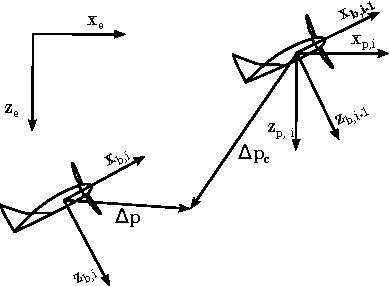
\includegraphics[width=7.4cm]{frames.pdf}    % The printed column width is 8.4 cm.
\caption{Predecessor-follower geometry longitudinal}
\label{fig:frames}
\end{center}
\end{figure}
\subsection{Vehicle Model}
The continuous-time vehicle position dynamics w.r.t. the local inertial frame are given as follows:
\begin{align}
\mathbf{x}(t) &= (\mbf{p}(t) \; \mbf{v}(t))^T \\
\dot{\mathbf{p}}(t) &= \mbf{v}(t)\\
\dot{\mbf{v}}(t) &= \mbf{a}_{c}(t) + \mbf{a}_w(t) + \mbf{g}
\end{align}
where $\mbf{p} \in \mathbb{R}^3$ is the vehicle position, $\mbf{v} \in \mathbb{R}^3$ is its velocity w.r.t to the local inertial frame, $\mbf{a}_w(t) \in \mathbb{R}^3$ are accelerations induced by exogenous disturbances such as turbulence and another aircraft's wake, $\mbf{a}_{c}(t) \in \mathbb{R}^3$ are commanded accelerations and $\mbf{g} \in \mathbb{R}^3$ is the gravity vector in the local inertial frame.
It is assumed that load factors $\mbf{n}_c(t) = \frac{1}{|\mbf{g}|} \mbf{a}_c(t)$ are tracked by fast inner loop controllers in the vehicle body frame, leading to actual load factors $\mbf{n}(t) = \mbf{n}_c(t) + \mbf{n}_w(t)$ where $\mbf{n}_w(t) = \frac{1}{|\mbf{g}|} \mbf{a}_w(t)$ are unknown parasitic load factors introduced by exogenous disturbances and imperfect tracking. This leads to the following equation:
\begin{align}
\dot{\mbf{v}}(t) &= \mbf{R}_{eb}(t) |\mbf{g}|\mbf{n}_c(t) + \mbf{a}_w(t) + \mbf{g}
\label{eq:svmloadfactorlevel}
\end{align}
where $\mbf{R}_{eb}(t) \in \mathbb{R}^{3 \times 3}$ is the rotation matrix from the body frame to the NED frame. To simplify notation, it is assumed that the vehicle is trimmed, i.e. the nominal gravitational acceleration is compensated for by a trim control input $\mbf{n}_{c,0}(t) = \mbf{R}_{be}(t)(0 \; 0 \; -1)^{T}$ and a virtual control input is defined as follows:
\begin{align}
\mbf{u} (t)= \mbf{R}_{eb}(t) |\mbf{g}|(\mbf{n}_c(t) - \mbf{n}_{c,0}(t))	
\label{eq:defushort}
\end{align}
leading to
\begin{align}
\dot{\mbf{v}}(t) &= \mbf{R}_{eb}(t)|\mbf{g}|
(
\frac{1}{|\mbf{g}|}
(\mbf{R}_{be}(t) \mbf{u}(t) + \mbf{n}_{c,0}(t))
) + \mbf{a}_w(t) + \mbf{g}\\
\dot{\mbf{v}}(t) &= \mbf{u}(t) + \mbf{a}_w(t)
\label{eq:svmshort}
\end{align}
where now $\mbf{a}_w(t)$ also includes the small effects of imperfect knowledge of local gravitation. 
%???doubledefinition
Considering two UAS \idxFollower  and \idxPredecessor in a leader-follower configuration, this leads to relative position error dynamics
\begin{align}
\Delta \mbf{p}(t) &= \mbf{p}_\idxFollower(t) - \mbf{p}_\idxPredecessor(t) - \Delta \mbf{p}_c(t) \\
\Delta \dot{\mbf{p}}(t) &= \mbf{v}_{\idxFollower}(t) - \mbf{v}_{\idxPredecessor}(t) -  \Delta \dot{\mbf{p}}_c(t) \\
\Delta \dot{\mbf{v}}(t) &= \mbf{a}_\idxFollower(t) - \mbf{a}_\idxPredecessor(t) -  \Delta \ddot{\mbf{p}}_c(t)\\
{} &= \mbf{a}_{c,\idxFollower}(t) + \mbf{a}_{w,\idxFollower}(t)
 - \mbf{a}_\idxPredecessor(t) -  \Delta \ddot{\mbf{p}}_c(t)\\
{} &= \mbf{u}(t) + \mbf{a}_{w,\idxFollower}(t)
 - \mbf{a}_\idxPredecessor(t) -  \Delta \ddot{\mbf{p}}_c(t)
\end{align}
where $\Delta \mbf{p}(t)$ is the relative position error between UAS \idxFollower and its predecessor \idxPredecessor, $\Delta \mbf{v}(t)$ is the corresponding relative velocity error, $\Delta \mbf{p}_c(t)$ is the desired relative position to the predecessor, $\mbf{a}_\idxPredecessor(t)$ are accelerations of the predecessor w.r.t. to the NED frame.
The presented model is essentially of the same type as that used in  \cite{galzi2006uav} and provides the benefit of being vehicle-agnostic, as the specific vehicle dynamics are covered by the inner loop load factor controllers. On the other hand, perturbations $\mbf{a}_w$ and control input saturations are specific to a given vehicle and mission environment. It covers rotary wings as well as fixed wing UAS, which are the focus of this work.
\subsubsection{\textbf{Formation trajectory}}
The trajectory of the formation w.r.t. the local inertial frame is defined by the nominal trajectory of a virtual leader aircraft.
%Arbitrary shapes of the formation can be defined by the relative separation vectors $\Delta \mbf{p}$. 
\subsection{Input saturations}
For a fixed-wing UAS, the maximum load factors are naturally limited by the maximum thrust of the engine and the aerodynamic parameters of the aircraft, such as the stall angle $\alpha_{max}$, leading to saturations on the commanded load factors
\begin{align}
|{n}_{c, \idxAxis}(t)| \leq {N}_\idxAxis(t)
\label{eq:loadfactorsaturations}
\end{align}
with $\idxAxis = 1...3$. The load factor saturations $\mbf{N}(t)$ are time-varying since, including the engine thrust, they are function of the dynamic pressure $\bar{q}(t) = \frac{1}{2}\rho(t) V_a^2(t)$.
Saturations on the virtual control input (\ref{eq:defushort}) can be derived from (\ref{eq:loadfactorsaturations}) as follows:
\begin{align}
|{u}_\idxAxis(t)| &\leq {U}_\idxAxis(t) \\
\mbf{U}(t) &= \mbf{R}_{eb}(t) |\mbf{g}|(\mbf{N}(t)-\mbf{n}_{c,0}(t))
\label{eq:saturationsonU}
\end{align}
with $\idxAxis = 1...3$.
\section{Control design}
\label{sec:controldesign}
To benefit from significant aerodynamic performance gains, a follower aircraft needs to stay within a narrow spatial window roughly defined by (see e.g. \cite{jake2003f})
\begin{align}
-0.2 b < \Delta y' < -0.1 b \\
-0.1 b < \Delta z' < 0 
\label{eq:windowz}
\end{align}
with the wingspan $b$, while the longitudinal separation $\Delta x'$ is less critical due to slow vortex decay. The wingtip-to-wingtip separation vector $\Delta \mbf{p'} = ( \Delta x' \; \Delta y' \; \Delta z')^T$ is defined in the predecessor wind frame.
It is thus the control objective to drive the follower UAS into this window and stay within it.
\subsection{Information constraints}
It is assumed that only observations of the relative position and relative velocity vector between each UAS and its predecessor are available.
This allows for using low-cost vision-based relative localization techniques, which is a significant advantage taking into account the price range of GNSS RTK (Global Navigation Satellite System Real Time Kinematics) systems which would be required for localization with respect to the formation leader or other members of the formation that are not within the field of view of onboard vision sensors.
\subsection{Sliding surface design}
It is the control objective to drive the system to the sliding surface defined by
\begin{align}
\mbf{\sigma}(t) &= \mbf{G}\mbf{x}(t)
\label{eq:defsigmaconti-} \\
\mbf{x}(t) &=
\begin{pmatrix}
\Delta \mbf{p}(t)\\
\Delta \mbf{v}(t)
\end{pmatrix}
\end{align}
where $ \mbf{G} \in \mathbb{R}^{3 \times 6}$ and, once reached, to keep it on it for all subsequent times $t \geq t^*$. In the following, for the continuous-time case, the dependence on time is dropped for notational convenience. With
\begin{align}
\mbf{G} =
\begin{bmatrix}
\mbf{G}_1 \mbf{G}_2
\end{bmatrix}
\end{align}
the position error dynamics in sliding mode ($\mbf{\sigma} = \mbf{0}$) are the following 
\begin{align} 
\mbf{0}
&=
\begin{bmatrix}
\mbf{G}_1 \mbf{G}_2
\end{bmatrix}
\begin{pmatrix}
\Delta \mbf{p}\\
\Delta \mbf{v}
\end{pmatrix} \\
\mbf{\Delta} \dot{\mbf{p}}
&= - \mbf{G}_2^{-1} \mbf{G}_1 \mbf{\Delta} \mbf{p}
\label{eq:pdynwhilesliding}
\end{align}
Selecting $- \mbf{G}_2^{-1} \mbf{G}_1$ as Hurwitz ensures that $\Delta \mbf{p}$ asymptotically converges to zero while in sliding mode.\\
Mesh stability is a feature of a three-dimensional formation of vehicles that allows separation errors to stay locally contained (see e.g. \cite{Pant2002}). In other words, separation errors between a pair of vehicles are not amplified towards the neighboring vehicle pairs. More vehicles can be added to a mesh stable formation without changing the local controllers, providing scalability. It is a well known fact (\cite{Pant2002}) that linear controllers with local feedback information are mesh unstable.
While in sliding mode, the position error dynamics are by definition confined to (\ref{eq:pdynwhilesliding}), independently of adjacent separation errors, implying mesh stability if the system can be kept in sliding mode.
The open loop sliding variable dynamics are given as follows:
\begin{align}
\dot{{\sigma}} &= \mbf{G}
\begin{pmatrix}
\Delta \mbf{v} \\
\mbf{u} + \mbf{a}_{w,\idxFollower}
 - \mbf{a}_\idxPredecessor -  \Delta \ddot{\mbf{p}}_c
\end{pmatrix}\\
& = \mbf{G}
\begin{pmatrix}
\Delta \mbf{v} \\
 - \Delta \ddot{\mbf{p}}_c
\end{pmatrix} 
+ \mbf{G}
\begin{bmatrix}
{\mbf{0}}\\
{\mbf{I}}
\end{bmatrix}
(\mbf{u} + \mbf{a}_{w,\idxFollower} - \mbf{a}_\idxPredecessor) \\
&= \mbf{G} \mbf{\Phi}_k + \mbf{G} \mbf{B}(
\mbf{u}
 + {\mbf\Phi}_u)
\label{eq:sigmadynconti}\\
&= \mbf{\Phi}'_k + \mbf{\Phi}'_u + \mbf{u}'
\label{eq:sigmadyncontishort}
\end{align}
The  desired relative position $\Delta \mbf{p}_c$ and its first and second derivatives are communicated to each follower. Accelerations of the predecessor $\mbf{a}_{k-1}$ as well as exogenous perturbations $\mbf{a}_{w, \idxFollower} $ acting on the vehicle $i$ are assumed to be unknown but bounded. For notational convenience they are lumped into the disturbance vector $\mbf{\Phi}_u$
\begin{align}
\mbf{\Phi}_u &= \mbf{a}_{w,\idxFollower} - \mbf{a}_\idxPredecessor
\end{align}
while the known perturbations are redefined as $\mbf{\Phi}_k$
\begin{align}
\mbf{\Phi}_k &= 
\begin{pmatrix}
\Delta \mbf{v} \\
 - \Delta \ddot{\mbf{p}}_c
\end{pmatrix} 
\end{align}
further defining
\begin{align}
\mbf{u}' &= \mbf{GB}\mbf{u}
\label{eq:defu}\\
\mbf{\Phi}_k' &= \mbf{G}\mbf{\Phi}_k \\
\mbf{\Phi}_u' &= \mbf{GB}\mbf{\Phi}_u
\end{align}
Note that all perturbations are assumed to satisfy the matching condition.
The three axes are considered decoupled by the inner load factor controllers, allowing for SISO design.
Saturations on the virtual control input (\ref{eq:defu}) can be derived from (\ref{eq:saturationsonU}) as
\begin{align}
|{u}'_\idxAxis| &\leq {U}'_\idxAxis \\
\mbf{U}' &= \mbf{GB} \mbf{R}_{eb} |\mbf{g}|(\mbf{N}-\mbf{n}_{c,0})
\end{align}
for $\idxAxis=1...3$.
\subsection{TSCSMC design}
Since the inner loop load factor controllers cannot track discontinuous reference signals, a continuous control signal is mandatory.
The system (\ref{eq:sigmadyncontishort}) is of relative degree $\mbf{r} = (1 \; 1 \; 1)^T$, thus continuous-time Super-Twisting Sliding Mode controllers (STCSMC, see e.g. \cite{shtessel2014sliding}) can be applied, providing continuous control signals.
We apply the controller presented in \cite{galzi2006uav} extending it trivially from 2D to 3D tracking.
The STCSMC controller is then given by
\begin{align}
u_\idxAxis' = \alpha_\idxAxis |\sigma_\idxAxis|^{1/2}\mathrm{sign(\sigma_\idxAxis)} + \beta_\idxAxis \int \mathrm{sign}(\sigma_\idxAxis) dt
\end{align}
where $\idxAxis = 1...3$ indicates the three decoupled axes. Adding a term that eliminates the known disturbances ${\Phi}_{k,i}'$ as in \cite{galzi2006uav}
\begin{align}
u_\idxAxis' = \alpha_\idxAxis |\sigma_\idxAxis|^{1/2}\mathrm{sign(\sigma_\idxAxis)} + \beta_\idxAxis \int \mathrm{sign}(\sigma_\idxAxis) dt - {\Phi}'_{k,\idxAxis}
\end{align}
leads to closed loop $\mbf{\sigma}$ dynamics of
\begin{align}
\dot{\sigma}_\idxAxis = \alpha_\idxAxis |\sigma_\idxAxis|^{1/2}\mathrm{sign(\sigma_\idxAxis)} + \beta_\idxAxis \int \mathrm{sign}(\sigma_\idxAxis) dt + \Phi_{u,\idxAxis}'
\end{align}
Provided the disturbances $\Phi'_{u,\idxAxis}$ are bounded by $\Phi'_{u,\idxAxis} \leq L_\idxAxis$ controller parameters that fulfill
\begin{align}
\alpha_\idxAxis = 1.5 \sqrt{L_\idxAxis}
\label{eq:csmcgainconditionalpha}\\
\beta_\idxAxis = 1.1 L_\idxAxis
\label{eq:csmcgainconditionbeta}
\end{align}
for $\idxAxis=1...3$ drive the system into 2-sliding mode, i.e. $\dot{\sigma} = \sigma = 0$ in finite time. The reaching time is bounded by $t_\idxAxis^* \leq \frac{7.6 \sigma_\idxAxis(0)}{\beta_\idxAxis - L_\idxAxis}$, see \cite{galzi2006uav}.
The actual control input $\mbf{n}_c$ is computed from (\ref{eq:defu}, \ref{eq:defushort}) as
\begin{align}
\mbf{n}_c = \frac{1}{|\mbf{g}|} \mbf{R}_{be}(\mbf{GB})^{-1} \mbf{u}' + \mbf{n}_{c,0}
\end{align}
using $\mbf{R}_{eb}^{-1} = \mbf{R}_{eb}^{T} = \mbf{R}_{be}$
%\subsubsection{Sliding condition}
%
%Ideal sliding mode controllers completely eliminate the impact of matched perturbations by injecting a control input that perfectly follows them. To verify that the system can actually be kept in sliding mode after the reaching phase despite limited control resources, the equivalent control is computed, i.e. the control that would satisfy the sliding condition if unknown perturbations were known. For (\ref{eq:sigmadyncontishort}), it results to
%
%\begin{align}
%{u}_{eq,i} = - {\Phi}_{k,i}' - {\Phi}_{u,i}'
%\end{align}
%
%Provided that
%\begin{align}
%\mbf{\Phi}_k'
%&= \mbf{G}
%\begin{pmatrix}
%\Delta \mbf{v} \\
% \Delta \ddot{p}_c
%\end{pmatrix}
%&\leq
%\mbf{M}\\
% &{\Phi}_{k,i}'
% &\leq
%{M}_i
%\end{align}
%
%with $\mbf{M} \in \mathbb{R}^3$ and $i=1...3$, $u_{eq,i}$ is bounded by
%
%\begin{align}
%|u_{eq,i}| \leq M_i + L_i
%\end{align}
%
%The unknown perturbations $\Phi_{u,i}$ are driven by exogenous disturbances $a_{w,i}$ and acceleration of the predecessor $a_{k-1,i}$.
%
%!!!Finish equivalent control part

%Those being bounded by (see (\ref{eq:svmloadfactorlevel}))
%
%\begin{align}
%|a_{w,i}| &\leq A_{w,i} \\
%|a_{k-1,i}| &\leq ||\mbf{g}|\mbf{n}_c| + |\mbf{a}_w| + |\mbf{g}|
%\end{align}

%\begin{align}
%u_i &= u_1 +  u_2
%\label{eq:STSMC}\\
%\dot{u}_1 &=
%\begin{array}{lr}
%-u \hspace{2em}
%& \mathrm{if} \; |u| > U\\
%-\alpha \mathrm{sign}(\sigma) \hspace{2em}
%& \mathrm{if} \; |u| \leq U\\
%\end{array} \\
%{u}_2 &=
%\begin{array}{lr}
%-\lambda |\sigma_0|^{1/2} \mathrm{sign}(\sigma)
% \hspace{2em}
%& \mathrm{if} \; |\sigma| > \sigma_0\\
%-\lambda |\sigma|^{1/2} \mathrm{sign}(\sigma)
% \hspace{2em}
%& \mathrm{if} \; |\sigma| \leq \sigma_0\\
%\end{array}
%\end{align}
\subsubsection{\textbf{Discretization}}
For implementation, the STCSMC is sampled with a zero-order hold scheme, leading to the Time-sampled Continuous Sliding Mode controller (TSCSMC). 

%\begin{align}
%u_i(\idxSample) = \alpha_i |\sigma_i(\idxSample)|^{1/2}\mathrm{sign(\sigma_i(\idxSample))} + \beta_i
%T
%\sum_{p=0}^{k}
%\mathrm{sign}(\sigma_i(p))
%\end{align}

\subsection{DSMC}
Designing a sliding mode controller in the discrete time domain allows to take sampling time effects into account right from the beginning. \\
The $\sigma$ dynamics resulting from (\ref{eq:sigmadyncontishort}) assuming forward Euler discretization are

\begin{align}
{{\sigma}}(\idxSample+1)
&=
{{\sigma}}(\idxSample)
+
T(
\mbf{\Phi}'_k(\idxSample) + \mbf{\Phi}'_u(\idxSample) + \mbf{u}'(\idxSample))
\label{eq:sigmadyndiscrete}
\end{align}

Since a discrete controller has no control over what happens to the continuous system between sampling instants, ideal sliding mode is not achievable. It is however possible to drive the system into so-called quasi-sliding mode, defined by the control objective

\begin{align}
|{\sigma}_\idxAxis (\idxSample)| \leq \mbf{\epsilon}_\idxAxis
\label{eq:controlobjective}
\end{align}

for $\idxAxis=1...3$, for all $\idxSample \geq \idxSample^*$ where $\epsilon_\idxAxis$ are the widths of the quasi-sliding mode boundary layer and $\idxSample^*$ is the first sample for which \ref{eq:controlobjective} is satisfied, i.e. when the system transitions from the reaching phase into quasi-sliding mode.
The proposed DSMC is based on ideas presented by the authors of \cite{monsees2001discrete}
The following simple linear reaching law (proposed e.g. by \cite{Spurgeon1992}) ensures asymptotic convergence to the sliding surface
\begin{align}
\mbf{\sigma}(\idxSample+1) = \mbf{\Psi} \mbf{\sigma}(\idxSample)
\label{eq:reachinglaw}
\end{align}
with a diagonal $\mbf{\Psi} \in \mathbb{R}^{3 \times 3}, 0 < \Psi_{\idxAxis,\idxAxis} < 1$ for $\idxAxis=1...3$. The choice of $\mbf{\Psi}$ allows to trade off control effort and reaching time.
Since (\ref{eq:reachinglaw}) is equivalent to
\begin{align}
|\mbf{\sigma}(\idxSample+1)| = \mbf{\Psi} |\mbf{\sigma}(\idxSample)|
\end{align}
the norm of the sliding variable decreases with every time step, indicating convergence to the sliding surface. 

\subsubsection{Remark} As mentioned in \cite{monsees2001discrete}, a Lyapunov function does not - as in the continuous case - provide enough constraints to drive the system to the sliding surface without overshoot. This is due to the fact that a Lyapunov function typically only constrains the direction of the system's motion - towards the sliding surface - but not the magnitude of the next discrete step towards it. 

The control input $\mbf{u}(\idxSample)$ required to drive the system (\ref{eq:sigmadyndiscrete}) according to the reaching law (\ref{eq:reachinglaw}) can be computed from the open-loop $\mbf{\sigma}$ dynamics to
\begin{align}
\mbf{u}'(\idxSample) &= \frac{1}{T}(\mbf{\Psi} - \mbf{I})\mbf{\sigma}(\idxSample) - \mbf{\Phi}_k' - \tilde{\mbf{\Phi}}_u'
\end{align}
Note that $\mbf{u}'(\idxSample)$ contains an estimate of the unknown perturbations $\tilde{\mbf{\Phi}}'_u(\idxSample) = \mbf{\Phi}'_u(\idxSample) + \Delta \mbf{\Phi}'_u(\idxSample)$. 
A simple way to obtain an estimate of the unknown disturbances is from the previous sample by
\begin{align}
\mbf{\Phi}_u(\idxSample-1) &=
\mbf{\sigma}(\idxSample)
-
\mbf{\sigma}(\idxSample-1)
-
T
(\mbf{\Phi}'_k(\idxSample-1) + \mbf{u}'(\idxSample-1))
\end{align}
Assuming that the disturbance rate is bounded by $|\frac{d \mbf{\Phi}'}{dt}| \leq \delta \Phi'_u$, assuming $\mbf{\Phi}'(\idxSample) = \mbf{\Phi}'(\idxSample-1)$ and a first-order approximation introduces an error $\Delta \mbf{\Phi}'_u(\idxSample)$ that is bounded by $|\Delta \mbf{\Phi}'_u(\idxSample)| \leq T \delta \Phi'_u $.\\
Closing the loop, one obtains
\begin{align}
\mbf{\sigma}(\idxSample+1) &= \mbf{\Psi} \mbf{\sigma}(\idxSample) +
T \Delta \mbf{\Phi}'_u(\idxSample)
\end{align}
Note that the reaching law (\ref{eq:reachinglaw}) can not be followed due to the bounded estimation error $\Delta \mbf{\Phi}'_u(\idxSample)$. Instead, assuming that initially the system is outside the quasi-sliding mode band, it will approach the sliding surface at least as long as
\begin{align}
(\mbf{I} - \mbf{\Psi}) \mbf{\sigma}(\idxSample) & > T^2 \delta \Phi'_u
\end{align}
This defines the vector of maximum boundary layer thicknesses as
\begin{align}
\epsilon &=
(\mbf{I} - \mbf{\Psi})^{-1} T^2 \delta \Phi'_u
\label{eq:achievableepsilon}
\end{align}
Once $\mbf{\sigma}$ has entered the boundary layer defined by $\mbf{\epsilon}$, it stays within it. This can be shown by considering an arbitrary $\mbf{\sigma}(k) < \mbf{\epsilon}$.\\ 
By writing the closed loop dynamics as
\begin{align}
\mbf{\sigma}(\idxSample+1) &= 
\mbf{\sigma}
(
\idxSample) -
(\mbf{I} - \mbf{\Psi}) 
\mbf{\sigma}(k)
+
T \Delta \mbf{\Phi}'_u(\idxSample)
\end{align}
the component wise maximum step away from the sliding surface is bounded by
\begin{align}
|{\sigma}_\idxAxis(\idxSample+1) - {\sigma}_\idxAxis(\idxSample)|
&\leq (1-\Psi_{\idxAxis, \idxAxis})\epsilon_\idxAxis - (1-\Psi_{\idxAxis, \idxAxis})|\sigma_\idxAxis| \\
&\leq (1-\Psi_{\idxAxis, \idxAxis})(\epsilon_\idxAxis - |\sigma_\idxAxis|)
\end{align}
which is smaller than the distance from the current ${\sigma_\idxAxis}$ to the boundary layer surface since
\begin{align}
(1-\Psi_{\idxAxis, \idxAxis})(\epsilon_\idxAxis - |\sigma_\idxAxis|) < \epsilon_\idxAxis - |\sigma_\idxAxis|
\end{align}
for $\idxAxis = 1...3$.

Note that with (\ref{eq:achievableepsilon}), the boundary layer thickness depends quadratically on the sampling time. Note also that to minimize the boundary layer thickness, small diagonal entries of $\mbf{\Psi}$ are desirable. At the same time, the initial system state may be far off the sliding surface, limiting the choice of $\mbf{\Psi}$ to avoid control input saturations. 
\subsection{PDSMC}
To join these conflicting requirements, we propose a time-varying reaching law, leading to a Predictive Discrete Sliding Mode Controller (PDSMC). As the linear reaching law (\ref{eq:reachinglaw}) it enforces a contraction of $\mbf{\sigma}$ towards the sliding surface at each time step. In contrast to (\ref{eq:reachinglaw}), the step towards the sliding surface is maximized by solving at each time step the optimization problem
\begin{align}
& \underset{\mbf{u'}(\idxSample)}{\text{minimize}}
& & |\mbf{\sigma}(\idxSample+1)| 
\label{eq:optimprob} \\
& \text{subject to}
& & \mbf{U}'_{min}(\idxSample) \leq \mbf{u'}(\idxSample) \leq \mbf{U}'_{max}(\idxSample) 
\end{align}
In practice this is equivalent to choosing a smaller reaching matrix $\mbf{\Psi}$ when closer to the sliding surface, leading to tighter bounds on the boundary layer thickness and thus reducing the maximum tracking error.\\
As an advantage of this approach, inner loop input rate saturations can be taken into account by defining 
\begin{align}
|\mbf{u'}(\idxSample) - \mbf{u'}(\idxSample-1)| \leq \mbf{\Delta U}'
\end{align}
which can be enforced by setting
\begin{align}
\mbf{U}'_{max}(\idxSample) = sat(\mbf{u}(\idxSample-1) + \mbf{\Delta U}', -\mbf{U}', \mbf{U}') \\
\mbf{U}'_{min}(\idxSample) = sat(\mbf{u}(\idxSample-1) - \mbf{\Delta U}', -\mbf{U}', \mbf{U}') 
\end{align}
Since $\mbf{\sigma}(\idxSample + 1)$ linearly depends on $\mbf{u}'(\idxSample)$, (\ref{eq:optimprob}) can efficiently be solved as quadratic program.
\section{Simulations}
\label{sec:simulations}
The TSCSMC and the DSMC with the linear and the predictive reaching law have been evaluated in a simulation environment implemented in Matlab\textsuperscript{\tiny \textregistered}/Simulink\textsuperscript{\tiny \textregistered}. In the proposed simulation scenarios, the closed loop vehicle dynamics have been integrated with a forward Euler scheme. While three-dimensional predecessor tracking is performed, only the vertical position tracking error $\Delta p_3$ is considered here for clarity. No sensor noise is considered in this work.
\subsection{Controller parameters}
For the TSCSMC, the controller gains are computed according to (\ref{eq:csmcgainconditionalpha}, \ref{eq:csmcgainconditionbeta}).\\
For the DSMC, the entries of the reaching matrix $\mbf{\Psi}$ are selected on line to stay within control input limits given the initial error state.\\
For the PDSMC, only input and input rate saturations need to be defined.

%, requiring the bounds $L_\idxAxis$ on the maximum unknown perturbations $\Phi'_{u,\idxAxis}$ which are driven by exogenous disturbances $a_{w,\idxAxis}$ and acceleration of the predecessor $a_{\idxPredecessor,\idxAxis}$.

%These being bounded by

%\begin{align}
%|a_{w,\idxAxis}| &\leq A_{w,\idxAxis} \\
%|a_{\idxPredecessor,\idxAxis}| &\leq A_{\idxPredecessor,\idxAxis}
%\end{align}

%for $\idxAxis = 1...3$, the bounds on $|a_{w,\idxAxis}|$ have been obtained empirically from a time series representing 1h of simulated Dryden turbulence at the position of maximum incremental lift in the predecessor's wake filtered by closed loop inner load factor controllers. \\
%The bounds $A_{k-1,i}$ are less obvious, since they depend on the closed-loop behavior of the predecessor. Assuming that the control inputs of the predecessor stay within their saturation limits, i.e. 
%\begin{align}
%-{U}_i < \mbf{u}_{\idxPredecessor, \idxAxis} < {U}_i 
%\label{eq:assumptionpredecessorinputs}
%\end{align}

%Now since

%\begin{align}
%\mbf{a}_{\idxPredecessor} = \mbf{u}_{\idxPredecessor} + \mbf{a}_{w, \idxPredecessor}
%\end{align}

%$\mbf{a}_{\idxPredecessor}$ is bounded by

%\begin{align}
%|a_{\idxPredecessor,\idxAxis}| &\leq U_\idxAxis + A_{w,\idxAxis}
%\end{align}

%leading to 

%\begin{align}
%L_\idxAxis &= U_\idxAxis + 2 A_{w,\idxAxis}
%\label{eq:boundLi}
%\end{align}

%\textbf{Remark}: From (\ref{eq:boundLi}) is becomes clear that no guarantees can be given for the system to stay in sliding mode at all times under the assumption \ref{eq:assumptionpredecessorinputs}. This is due to the fact that the assumption \ref{eq:assumptionpredecessorinputs} allows the predecessor \idxPredecessor to apply maximum accelerations that, if at the same time disturbances $\mbf{a}_{w, \idxAxis}$ act on the predecessor, cannot be followed by the follower \idxFollower. Formally this can be checked by computing the equivalent control and its bounds that result from the sliding condition $\dot{\mbf{\sigma}} = \mbf{0}$ as

%\begin{align}
%{u}'_{eq,\idxAxis} &= - {\Phi}'_{k, \idxAxis} - {\Phi}'_{u, \idxAxis}\\
%|{u}'_{eq,\idxAxis}| &\leq {\Phi}'_{k, \idxAxis, max} + L_\idxAxis \\
%{} &\leq {\Phi}'_{k, \idxAxis, max} + U_\idxAxis + 2 A_{w,\idxAxis}
%\end{align}

%Note that the bounds on $u_{eq,\idxAxis} $ exceed the control saturations $U_\idxAxis$.

%For the first vehicle pair, which is formed by the virtual leader and the first aircraft, the predecessor control input bounds expressed by (\ref{eq:assumptionpredecessorinputs}) can easily be tightened by limiting the second derivative of the virtual leader's trajectory. For the following vehicle pairs, control inputs depend on the sampled closed loop behavior of the controller, which is quite different for the two controllers compared here, as we will see in section \ref{sec:simulations}.

%\textcolor{red}{!!!Explain what happens to following pairs, since control input of i becomes predecessor commanded acceleration of i+1 -> fundamentally not mesh stable. Expected result: tracking accuracy can be guaranteed for a certain number of pairs, once exceeded, controls saturate}
\subsection{Disturbance models}

\subsubsection{\textbf{Wake vortex disturbances}}

\begin{figure}
\begin{center}
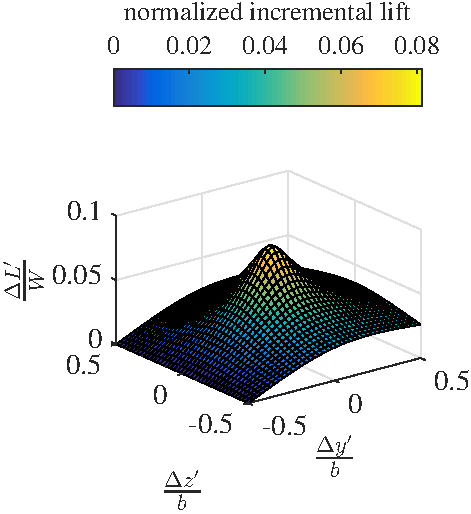
\includegraphics[width=8.4cm]{incrementallift}    % The printed column width is 8.4 cm.
\caption{Normalized incremental lift predicted by modified Horseshoe Vortex Model for $\Delta x' = 2b$. Note that $\Delta x', \Delta y', \Delta z'$ are wingtip to wingtip separations}
\label{fig:HSVMincrementalift}
\end{center}
\end{figure}
A variety of approaches has been proposed to simulate the effects of trailing vortices on the following UAS, mostly based on modified Horseshoe Vortex models (HVM) (e.g. \cite{Hummel1982}) or Vortex Lattice methods (VLM) (e.g. \cite{Saban2009}). For the purpose of this work, a HVM with modified core model presented in (\cite{dogan2005modeling}) is used. It is reported to provide predictions that are in good agreement with both VLM models and wind tunnel measurements while being of great simplicity. In the vertical channel, the model predicts incremental aerodynamic lift perturbations as a function of the separation vector between a UAS and its predecessor, see fig. \ref{fig:HSVMincrementalift} for an example.
\subsubsection{\textbf{Atmospheric turbulence}}
Atmospheric turbulence time series are generated according to the Dryden turbulence spectrum. The induced velocities are filtered by transfer functions corresponding to closed loop LQR load factor controllers designed for a small UAS ($b=2.6 \, m$). An ambient headwind of 20\% of the airspeed ($V_a = 15 \, \frac{m}{s}$) is assumed. See fig. \ref{fig:nwztimeseries} for an example time series of the resulting total vertical load factor perturbations $n_{w,3} = \frac{a_{w,3}}{|\mbf{g}|}$.
\begin{figure}
\begin{center}
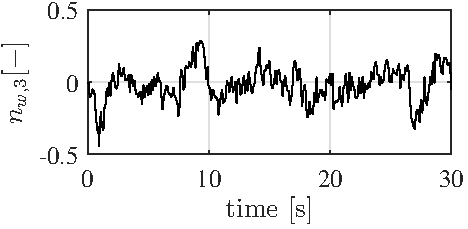
\includegraphics[scale=1]{nwz-timeseries}    % The printed column width is 8.4 cm.
\caption{ Example time series of vertical load factor disturbances}
\label{fig:nwztimeseries}
\end{center}
\end{figure}
\subsection{{Benchmark maneuver}}
To evaluate the control performance, a benchmark maneuver is performed by a formation of 5 UAS (vehicle index $\#\idxFollower$, the virtual leader has index 0 and is not shown). The vehicles start in a staggered formation with relative separations of $\Delta \mbf{p}_{c,j} = \mbf{R}_{el} (-2b \; b \; b)^T$ for $j=1...4$, where $\mbf{R}_{ep}$ denotes the rotation matrix from the predecessor velocity frame to the local inertial frame. At $t=5 \; s$ the vertical separation is driven to zero, i.e. $\Delta \mbf{p}_{c,j} = \mbf{R}_{el}(-2b \; b \; 0)^T$, and each UAS thus enters the zone of maximum incremental lift, see fig. \ref{fig:HSVMincrementalift}. This corresponds to the perturbation $\Delta \ddot{\mbf{p}}_c$. At $t=11 \;s$ the formation leader performs a climb by $10 \; m$, corresponding to the perturbation $\mbf{a}_{\idxPredecessor}$.
The benchmark maneuver is run with the TSCSMC controller at $T=10^{-3} \; s$ and all three controllers at $T=10^{-2} \; s$. The latter sampling frequency is considered realistic for implementation on board a small UAS. Note that tracking errors are normalized with the wingspan $b$ and control inputs with their saturation limits.\\
\subsection{Results}
The tracking error $\Delta z = \Delta p_3$ achieved by the TSCSMC as well the absolute vertical position and the control input are presented in Fig. \ref{fig:CSMC1000Hz} and Fig. \ref{fig:CSMC100Hz}. While tracking performance is very good in both cases and the tracking error $\Delta z$ stays well within the bounds indicated by (\ref{eq:windowz}), it degrades as expected with larger sampling times. Heavy input chattering appears and the control inputs run into saturation for large parts of the maneuver. In the realistic $T=10^{-2} \; s$ case, steady state tracking errors appear. 
\begin{figure}[h!]
\begin{center}
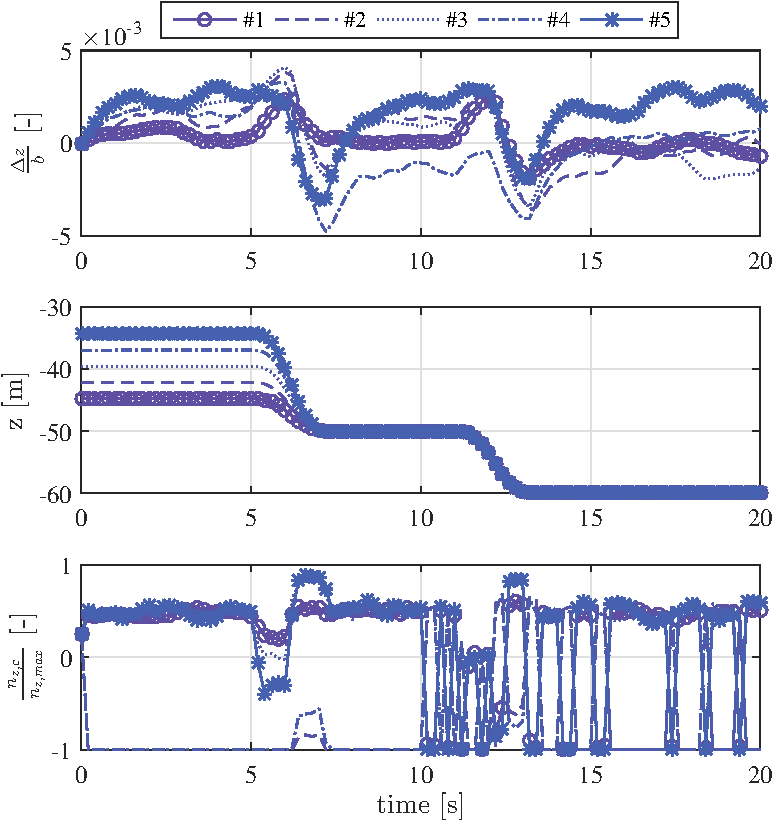
\includegraphics[width=\columnwidth,height=10cm]{TSCSMC-1000Hz-TIMESCALESEPARATION-turbulence=1}    % The printed column width is 8.4 cm.
\caption{TSCSMC controller $10^{-3} s$ sampling time}
\label{fig:CSMC1000Hz}
\end{center}
\end{figure}
\begin{figure} [h!]
\begin{center}
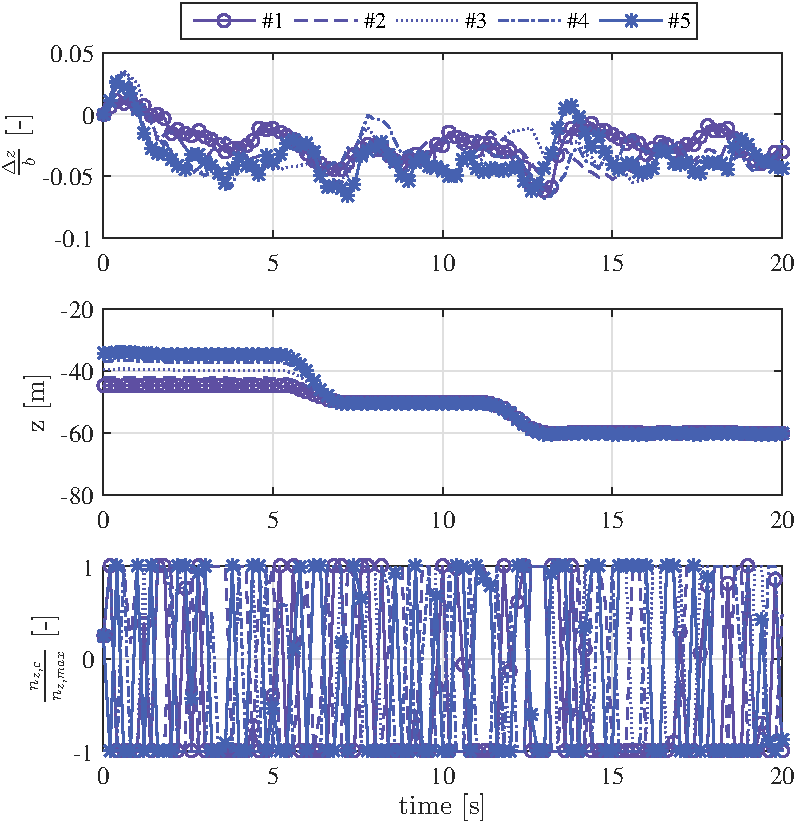
\includegraphics[width=\columnwidth,height=10cm]{TSCSMC-100Hz-TIMESCALESEPARATION-turbulence=1}    % The printed column width is 8.4 cm.
\caption{ TSCSMC controller $10^{-2} s$ sampling time}
\label{fig:CSMC100Hz}
\end{center}
\end{figure}
The DSMC, on the other hand, provides a tracking performance at $T = 10^{-2}$ comparable to that of the TSCSMC at $T = 10^{-3}$, see Fig. \ref{fig:DSMC100Hz}. The inputs stay at all times confined to the saturation limits and no chattering is to be observed. The PDSMC improves on this performance, see fig. \ref{fig:PDSMC100Hz}.
\begin{figure}[h!]
\begin{center}
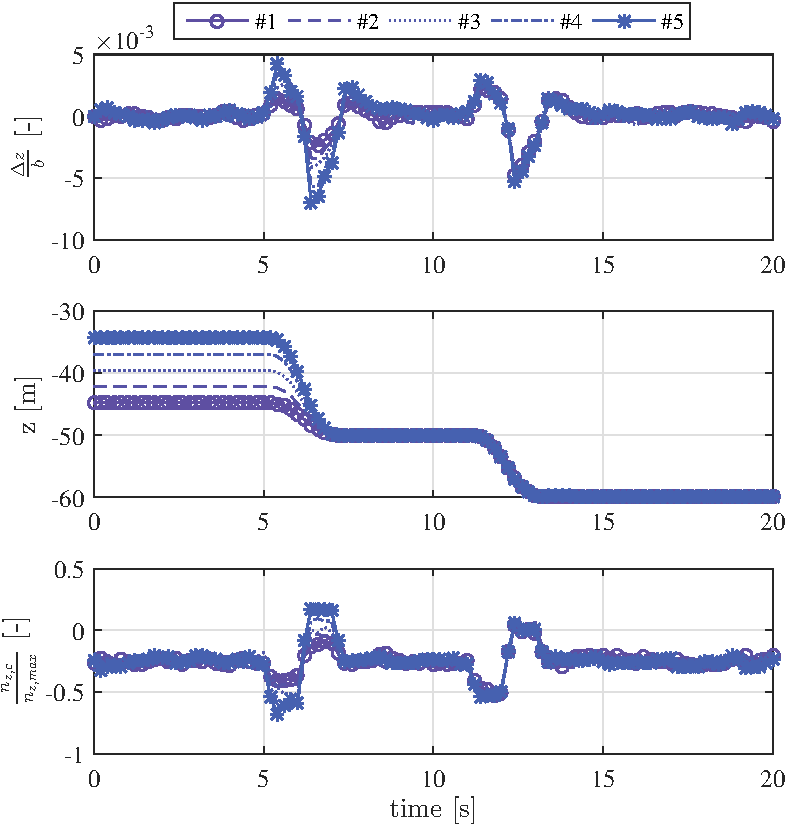
\includegraphics[width=\columnwidth,height=10cm]{DSMC-100Hz-TIMESCALESEPARATION-turbulence=1}    % The printed column width is 8.4 cm.
\caption{ DSMC controller $10^{-2} s$ sampling time}
\label{fig:DSMC100Hz}
\end{center}
\end{figure}
\begin{figure}[h!]
\begin{center}
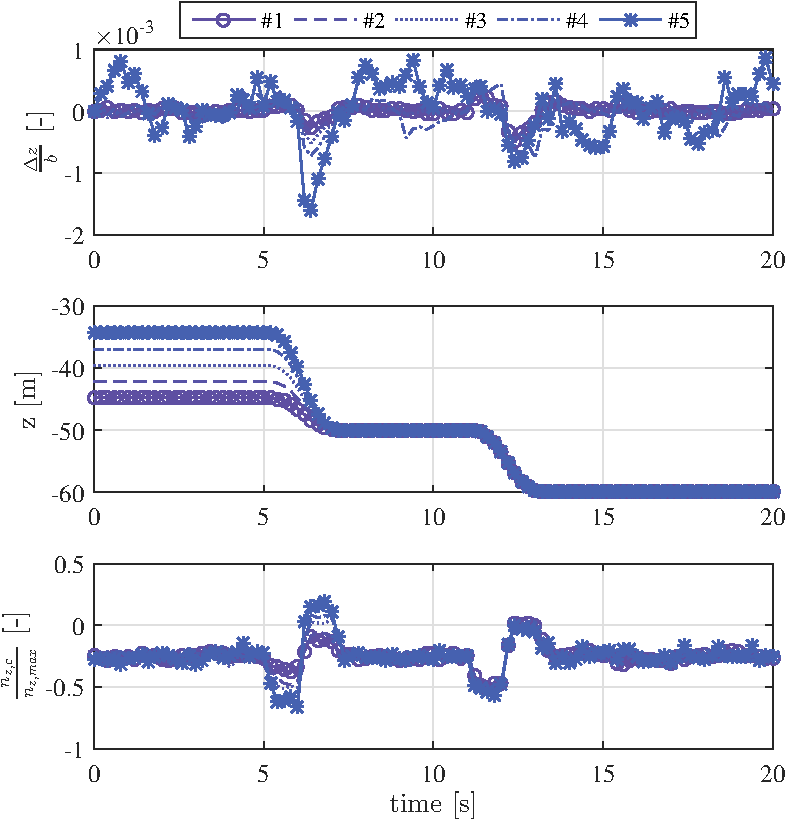
\includegraphics[width=\columnwidth,height=10cm]{PDSMC-100Hz-TIMESCALESEPARATION-turbulence=1}    % The printed column width is 8.4 cm.
\caption{ PDSMC controller $10^{-2} s$ sampling time}
\label{fig:PDSMC100Hz}
\end{center}
\end{figure}\\
This superior performance with respect to lower sampling times is systematically investigated by evaluating the maximum tracking error and the RMS tracking error over a grid of sampling times, as shown in Fig. \ref{fig:errorvssamplingtime}. Note that the RMS error and maximum error achieved by the DSMC stays for all sampling times below those of the TSCSMC and evolves more smoothly as the sampling time is varied. The PDSMC shows an evolution of the maximum error and RMS error similar to the DSMC while providing smaller error measures in both cases.\\
\begin{figure}[h!]
\begin{center}
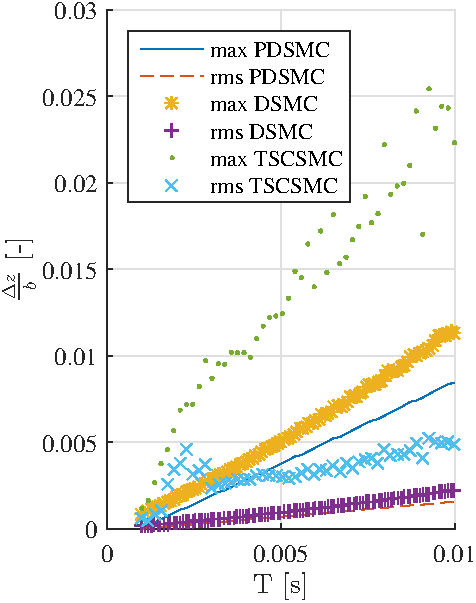
\includegraphics[width=0.9\columnwidth,height=9cm]{error-z-vs-samplingtime.pdf}    % The printed column width is 8.4 cm.
\caption{Vertical position error measures vs. controller sampling time for TSCSMC, DSMC, PDSMC}
\label{fig:errorvssamplingtime}
\end{center}
\end{figure}
Looking at figs.  \ref{fig:DSMC100Hz} and \ref{fig:PDSMC100Hz} the control error appears to increase with vehicle index, indicating mesh instability.\\
This is further confirmed by evaluating a formation of 30 vehicles, see fig. \ref{fig:errroamplification}. The maximum vertical control error as well as the RMS  error appear to depend roughly quadratically on the vehicle index.\\
This issue is well known for linear controllers (\cite{Pant2002}). It can be concluded that mesh stable sliding surfaces do not guarantee mesh stability in the discrete sampling case.
Note that the maximum tracking error for $\idxFollower = 30$ still satisfies the requirement (\ref{eq:windowz}).
%Thus while the formation is mesh unstable, due to the excellent overall tracking performance and low error amplification, tracking requirements are satisfied for modest formation sizes. It is desirable to investigate this aspect further and to provide analytical bounds on maximum tracking errors as function of the vehicle index. This could allow to drop the requirement of mesh stability and to replace it by a maximum formation size. In real world applications, formations are not unlimited in size
\begin{figure}[h!]
\begin{center}
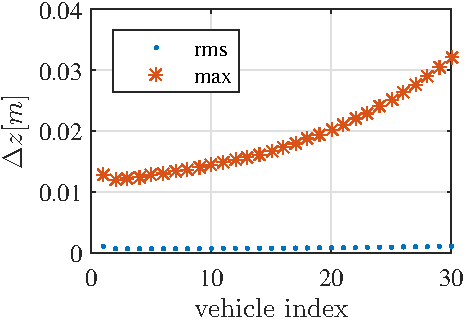
\includegraphics[width=\columnwidth,height=5cm]{erroramplification-DSMC-100Hz-TIMESCALESEPARATION-turbulence=1-turbulenceonlyfirstUAS}    % The printed column width is 8.4 cm.
\caption{ DSMC controller, vertical tracking error over vehicle index, $10^{-2} s$ sampling time}
\label{fig:errroamplification}
\end{center}
\end{figure}
{\section{Conclusion}
\label{sec:conclusion}
In this article, a discrete sliding mode controller using a novel predictive reaching law (PDSMC) for decentralized 3D trajectory tracking of multiple UAS has been presented and compared to a DSMC with linear reaching law and a discretized continuous time Super Twisting controller (TSCSMC). Analytical bounds on maximum sliding errors introduced by discrete sampling are provided for the DSMC.\\ 
Simulation results for a vertical benchmark maneuver illustrate the superior performance of both flavours of the DSMC. This is complemented by a simple and straightforward design procedure.\\ 
The authors intend to extend this promising approach to a broader class of systems by including inner loop dynamics and communication delays. It will be another focus of our future work to derive analytical bounds on the impact of sampling on mesh instability, an aspect only covered empirically in this work.
}

\bibliography{./bibliography/bibliographyPhD}             % bib file to produce the bibliography
                                                     % with bibtex (preferred)
                                                                                                                            % in the appendices.
\end{document}
